% !TeX document-id = {f19fb972-db1f-447e-9d78-531139c30778}
% !BIB program = biber

%\documentclass[handout]{beamer}
\documentclass[compress]{beamer}
\usepackage[T1]{fontenc}
\usetheme[block=fill,subsectionpage=progressbar,sectionpage=progressbar]{metropolis} 
\usepackage{graphicx}

\usepackage{wasysym}
\usepackage{etoolbox}
\usepackage[utf8]{inputenc}

\usepackage{pifont}

\usepackage{threeparttable}
\usepackage{subcaption}

\usepackage{tikz-qtree}
\usepackage{neuralnetwork}

\setbeamercovered{still covered={\opaqueness<1->{5}},again covered={\opaqueness<1->{100}}}


\usepackage{listings}

\lstset{
	basicstyle=\scriptsize\ttfamily,
	columns=flexible,
	breaklines=true,
	numbers=left,
	%stepsize=1,
	numberstyle=\tiny,
	backgroundcolor=\color[rgb]{0.85,0.90,1}
}



\lstnewenvironment{lstlistingoutput}{\lstset{basicstyle=\footnotesize\ttfamily,
		columns=flexible,
		breaklines=true,
		numbers=left,
		%stepsize=1,
		numberstyle=\tiny,
		backgroundcolor=\color[rgb]{.7,.7,.7}}}{}


\lstnewenvironment{lstlistingoutputtiny}{\lstset{basicstyle=\tiny\ttfamily,
		columns=flexible,
		breaklines=true,
		numbers=left,
		%stepsize=1,
		numberstyle=\tiny,
		backgroundcolor=\color[rgb]{.7,.7,.7}}}{}


% color-coded listings; replace those above 
\usepackage{xcolor}
\usepackage{minted}
\definecolor{listingbg}{rgb}{0.87,0.93,1}
\setminted[python]{
	frame=none,
	framesep=1mm,
	baselinestretch=1,
	bgcolor=listingbg,
	fontsize=\scriptsize,
	linenos,
	breaklines
	}


\usepackage[american]{babel}
\usepackage{csquotes}
\usepackage[style=apa, backend = biber]{biblatex}
\renewcommand*{\bibfont}{\tiny}


\usepackage{tikz}
\usetikzlibrary{shapes,arrows,matrix}
\usepackage{multicol}

\usepackage{subcaption}

\usepackage{booktabs}
\usepackage{graphicx}



\makeatletter
\setbeamertemplate{headline}{%
	\begin{beamercolorbox}[colsep=1.5pt]{upper separation line head}
	\end{beamercolorbox}
	\begin{beamercolorbox}{section in head/foot}
		\vskip2pt\insertnavigation{\paperwidth}\vskip2pt
	\end{beamercolorbox}%
	\begin{beamercolorbox}[colsep=1.5pt]{lower separation line head}
	\end{beamercolorbox}
}
\makeatother





\setbeamercolor{section in head/foot}{fg=normal text.bg, bg=structure.fg}


\newcommand{\instruction}[1]{\emph{\textcolor{gray}{[#1]}}}



\newcommand{\question}[1]{
	\begin{frame}[plain]
	\begin{columns}
		\column{.3\textwidth}
		\makebox[\columnwidth]{
			
\includegraphics[width=\columnwidth,height=\paperheight,keepaspectratio]{mannetje.png}}
		\column{.7\textwidth}
		\large
		\textcolor{orange}{\textbf{\emph{#1}}}
	\end{columns}
\end{frame}}


\tikzstyle{block} = [rectangle, draw, fill=blue!20, 
text width=5em, text centered, rounded corners, minimum height=4em]
\tikzstyle{line} = [draw]
\tikzstyle{pijltje} = [draw, -latex']
\tikzstyle{cloud} = [draw, ellipse,fill=red!20, node distance=3cm,
minimum height=2em, text width=4em, text centered,]


\setbeamercovered{transparent}

\addbibresource{../../resources/literature.bib}
\graphicspath{{../../resources/img/}}


\begin{document}

\title[Big Data and Automated Content Analysis]{\textbf{Big Data and Automated Content Analysis (12EC)} 
\\Week 8: »Supervised Approaches to Text Analysis«
\\Wednesday}
\author[Damian Trilling]{Damian Trilling\\ \footnotesize{d.c.trilling@uva.nl, @damian0604 \\}}
\date{April 6, 2022}
\institute[UvA CW]{UvA RM Communication Science}


\begin{frame}{}
	\titlepage
\end{frame}

\begin{frame}{Today}
	\tableofcontents
\end{frame}




\begin{frame}[standout]
This week, we will bring together our knowledge about machine learning and about BOW-representations of text.

It's the \textcolor{orange}{combination} of week 5 and week 6!
\end{frame}


\section{Supervised Machine Learning for Text Classification}

\begin{frame}{\cite{Boumans2016}: Types of Automated Content Analysis}
	\makebox[\columnwidth]{	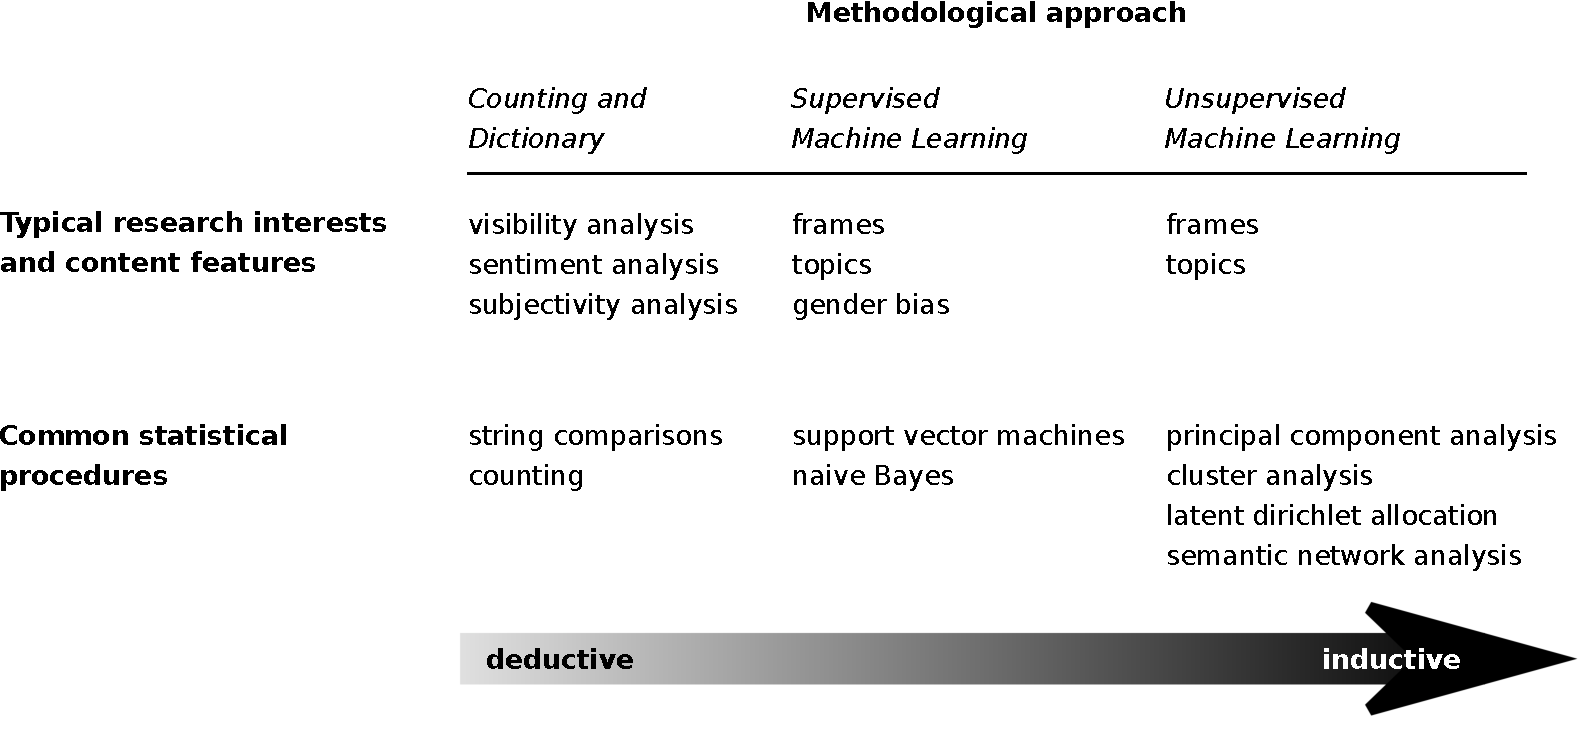
\includegraphics[width=\columnwidth,height=.8\paperheight,keepaspectratio]{boumanstrilling2016}}
\end{frame}


\begin{frame}{Recap: Supervised vs Unsupervised}
\begin{columns}[t]
\column{.5\textwidth}

\begin{block}<1-4>{Supervised machine learning}
  You have a dataset with both predictor and outcome (independent and dependent variables; features and labels) --- a \emph{labeled} dataset.
  \onslide<2>{
    \footnotesize{Think of regression: You measured \texttt{x1}, \texttt{x2}, \texttt{x3} and you want to predict \texttt{y}, which you also measured}}
\end{block}

\column{.5\textwidth}

\begin{block}<3->{Unsupervised machine learning}
  You have no labels. \onslide<4>{(\footnotesize{You did not measure \texttt{y})}}\\
  \onslide<5>{\textbf{You might already know \emph{some} techniques to figure out whether \texttt{x1}, \texttt{x2},\ldots \texttt{x\_i} co-occur} \begin{itemize}
    \item Principal Component Analysis (PCA) and Singular Value Decomposition (SVD)
    \item Cluster analysis
    \item Topic modelling (Non-negative matrix factorization and Latent Dirichlet Allocation)
    \item \ldots
    \end{itemize}}
\end{block}

\end{columns}

\end{frame}






\subsection{One step back: (Traditional) non-SML approaches}

\begin{frame}{Let's consider three tasks}
  For a given text (say, a news article, a press release, a review), determine the
  \begin{description}
  \item[sentiment] e.g., [positive|neutral|negative]
  \item[topic] e.g., [sports|economy|politics|entertainment|other]
  \item[frames] e.g., [economic|human|moral|conflict], or non-exclusive: economic = [0|1], human = [0|1], \ldots
  \end{description}
\end{frame}


\question{What would be the strengths and weaknesses of different approaches from the classification by \cite{Boumans2016} for each of these tasks?}


\question{Imagine using a dictionary-based (list of keywords, list of regular expressions, or similar) approach to these tasks. How does the design (length, inclusiveness, etc.) of this list influence precision and recall?}


\begin{frame}{Dictionary-based approaches for text classification}
  \begin{columns}[t]
    \column{.5\textwidth}
    \begin{block}{good for}
      \begin{itemize}
      \item distinct, manifest things (names of organizations, pronouns, swearwords (?), \ldots)
      \item little room for interpretation/misunderstandings etc.
      \item ``must-be-explainable-to-a-five-year-old''
      \end{itemize}
      \pause
    \end{block}
    \column{.5\textwidth}
    \begin{alertblock}{bad for}
      \begin{itemize}
      \item latent constructs and concepts
      \item implicit things
      \end{itemize}
      \pause
      Hence, \emph{not} state-of-the-art for
      \begin{itemize}
      \item topics
      \item frames
      \item sentiment
      \end{itemize}
    \end{alertblock}
  \end{columns}
\end{frame}


\begin{frame}[standout]
Let's discuss SML for text with the example of \textcolor{orange}{sentiment analysis}.
\end{frame}


\begin{frame}{From dictionary approaches to SML}
  \begin{itemize}[<+->]
  \item Early days of sentiment analysis: list of positive words, list of negative words, count what occurs most
  \item You can even \textit{buy} lists of words that are meant to measure constructs like ``positive emotions'' or even ``analytic'' or ``authentic'' language use from a psychologist (LIWC, \cite{Pennebaker2007})
  \end{itemize}
\end{frame}

\question{What do you think? Can this even work?}



\begin{frame}{Bag-of-words dictionary approaches to sentiment analysis}
  \begin{block}{con}
    \begin{itemize}
    \item simplistic assumptions
    \item e.g., intensifiers cannot be interpreted (``really'' in ``really good'' or ``really bad'')
    \item or, even more important, negations.
    \end{itemize}
  \end{block}
\end{frame}




\begin{frame}{Improving the BOW approach}
  \begin{block}{Example: Sentistrenght \parencite{Thelwall2012}}
    \begin{itemize}
    \item $-5\ldots-1$ and $+1\ldots+5$ instead of positive/negative
    \item spelling correction
    \item ``booster word list'' for strengthening/weakening the effect of the following word
    \item interpreting repeated letters (``baaaaaad''), CAPITALS and !!!
    \item idioms
    \item negation 
    \end{itemize}
	\end{block}
	VADER by \cite{Hutto2014} works in a similar way.
	\pause
	\footnotesize{Even though this is much less na\"ive than LIWC, for instance, the problem remains: Can we construct a dictionary that, \emph{irrespective of the context}, gives us a meaningful estimate of sentiment? }
\end{frame}





\begin{frame}[standout]
  Such an \textit{off-the-shelf} dictionary does not (and probably cannot) exist.
\end{frame}



\begin{frame}{\cite{Boukes2020}: Sentiment analysis of economic news}
  \makebox[\columnwidth]{
    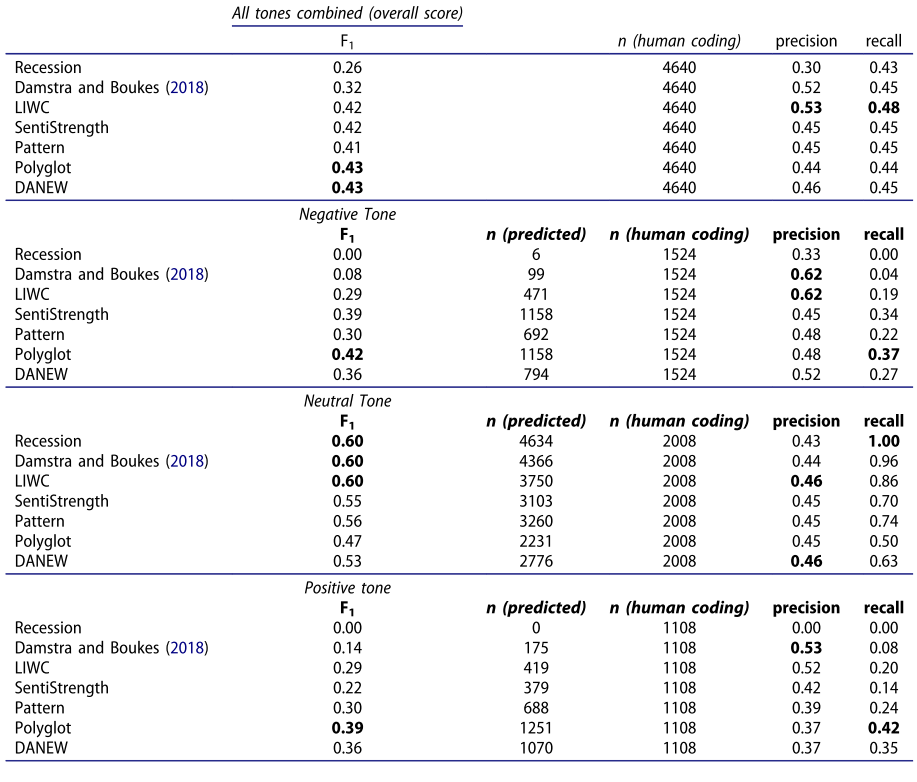
\includegraphics[width=\columnwidth,height=.8\paperheight,keepaspectratio]{boukes2019}}
\end{frame}


\begin{frame}{\cite{Boukes2020}: Sentiment analysis of economic news}
  \makebox[\columnwidth]{
    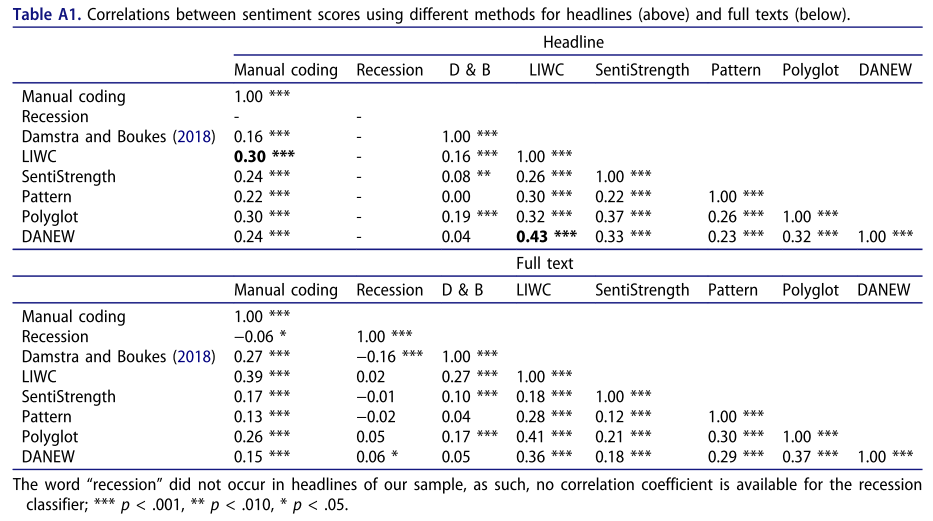
\includegraphics[width=\columnwidth,height=.8\paperheight,keepaspectratio]{boukes2019b}}
\end{frame}


\begin{frame}{\cite{Boukes2020}: Sentiment analysis of economic news}
  \begin{itemize}
  \item Dictionaries have low agreement with each other, and also with human coders
  \item Even their own dictionary didn't agree
  \item \textbf{This is not because these dictionaries are particularly bad!}. Main point: For such a complex and context-dependent task, a dictionary is just not the right tool.
  \end{itemize}
\end{frame}




\begin{frame}{\cite{VanAtteveldt2021}: Extending \cite{Boukes2020} with SML}
  ``manual coding (using undergraduate students) yields the
  best results 
  
  [\ldots] A good second place is taken by crowd coding [\ldots]  
  
  
  [\ldots] machine learning performs worse than both students' manual coding and crowd coding.
  Reaching $\alpha = 0.50$ for deep learning (CNN) and slightly worse for classical machine learning (SVM; $\alpha = 0.41$, NB; $\alpha = 0.40$), machine learning still performs significantly better than chance. However, since these results are lower than generally accepted levels of inter-coder reliability [\ldots]
  
  Finally, [\ldots] dictionaries [\ldots] perform worse than the machine
  learning results and much worse than manual annotation [\ldots] [and] approximate chance agreement''\end{frame}

  


\begin{frame}{\cite{Vermeer2019}: Satisfaction with brands}
  \makebox[\columnwidth]{
  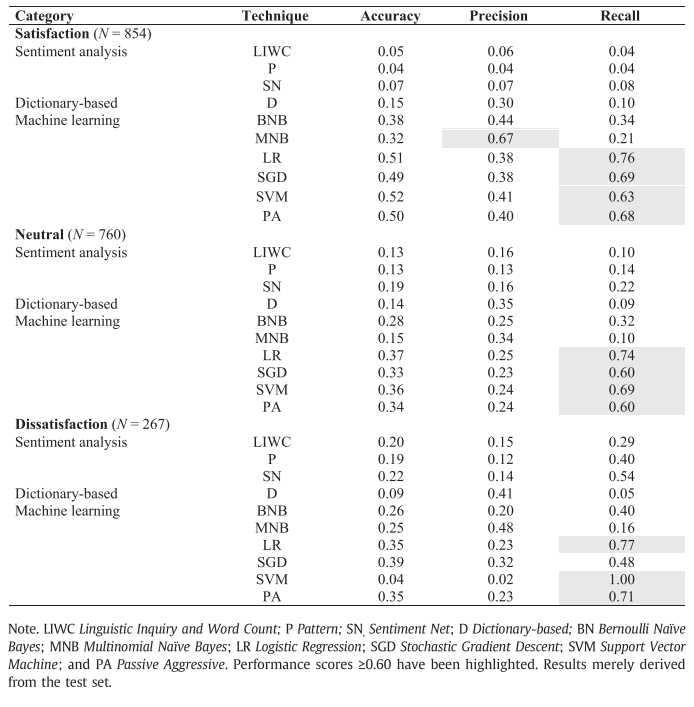
\includegraphics[width=\columnwidth,height=.8\paperheight,keepaspectratio]{vermeer2019}}
\end{frame}



\begin{frame}[standout]
  SML is no panacea, but the most promising approach to analyzing large quantities of texts. Don't believe off-the-shelf packages that claim to do the work for you.
  (For small datasets, just do it by hand.)
\end{frame}




\subsection{Diving into SML}

% Misschien hier maar wat nieuwere voorbeelden nemen?

\begin{frame}{SML to code frames and topics}
  \begin{block}{Some work by \cite{Burscher2014} and \cite{Burscher2015} }
    \begin{itemize}
    \item Humans can code generic frames (human-interest, economic, \ldots)
    \item Humans can code topics from a pre-defined list 
    \item<2->\textbf{But it is very hard to formulate an explicit rule} \\(as in: code as 'Human Interest' if regular expression R is matched)
    \end{itemize}
    \onslide<3>$\Rightarrow$ This is where you need supervised machine learning!
  \end{block}	
\end{frame}




{\setbeamercolor{background canvas}{bg=black}
  \begin{frame}[plain]
    \makebox[\linewidth]{
      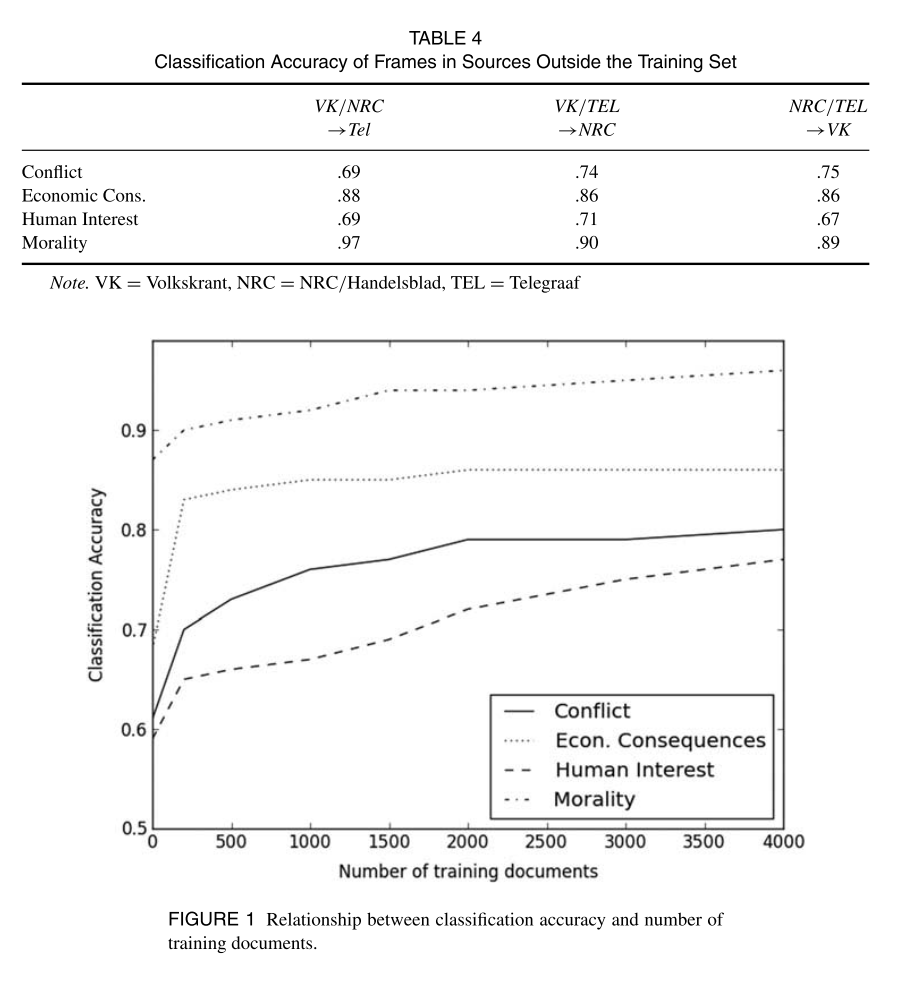
\includegraphics[width=\paperwidth,height=\paperheight,keepaspectratio]{burscher2014}}
  \end{frame}
  
  \begin{frame}[plain]
    \makebox[\linewidth]{
      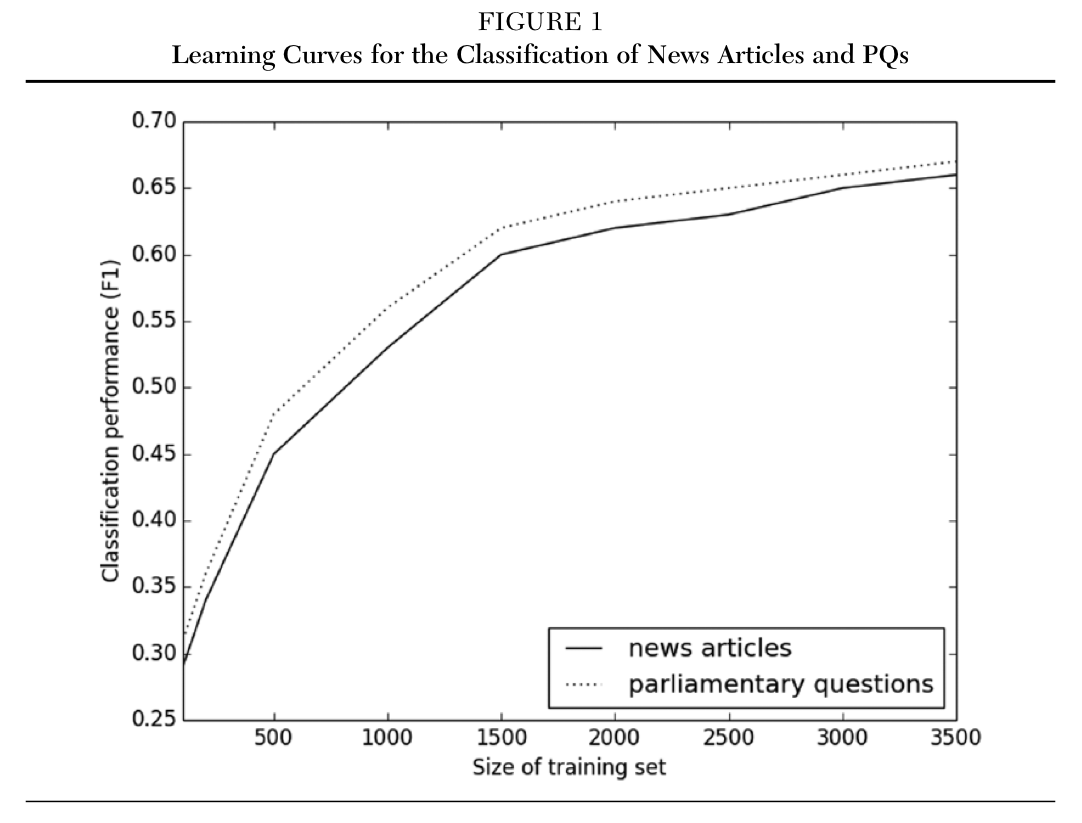
\includegraphics[width=\paperwidth,height=\paperheight,keepaspectratio]{burscher2015-a}}
  \end{frame}
  
  \begin{frame}[plain]
    \makebox[\linewidth]{
      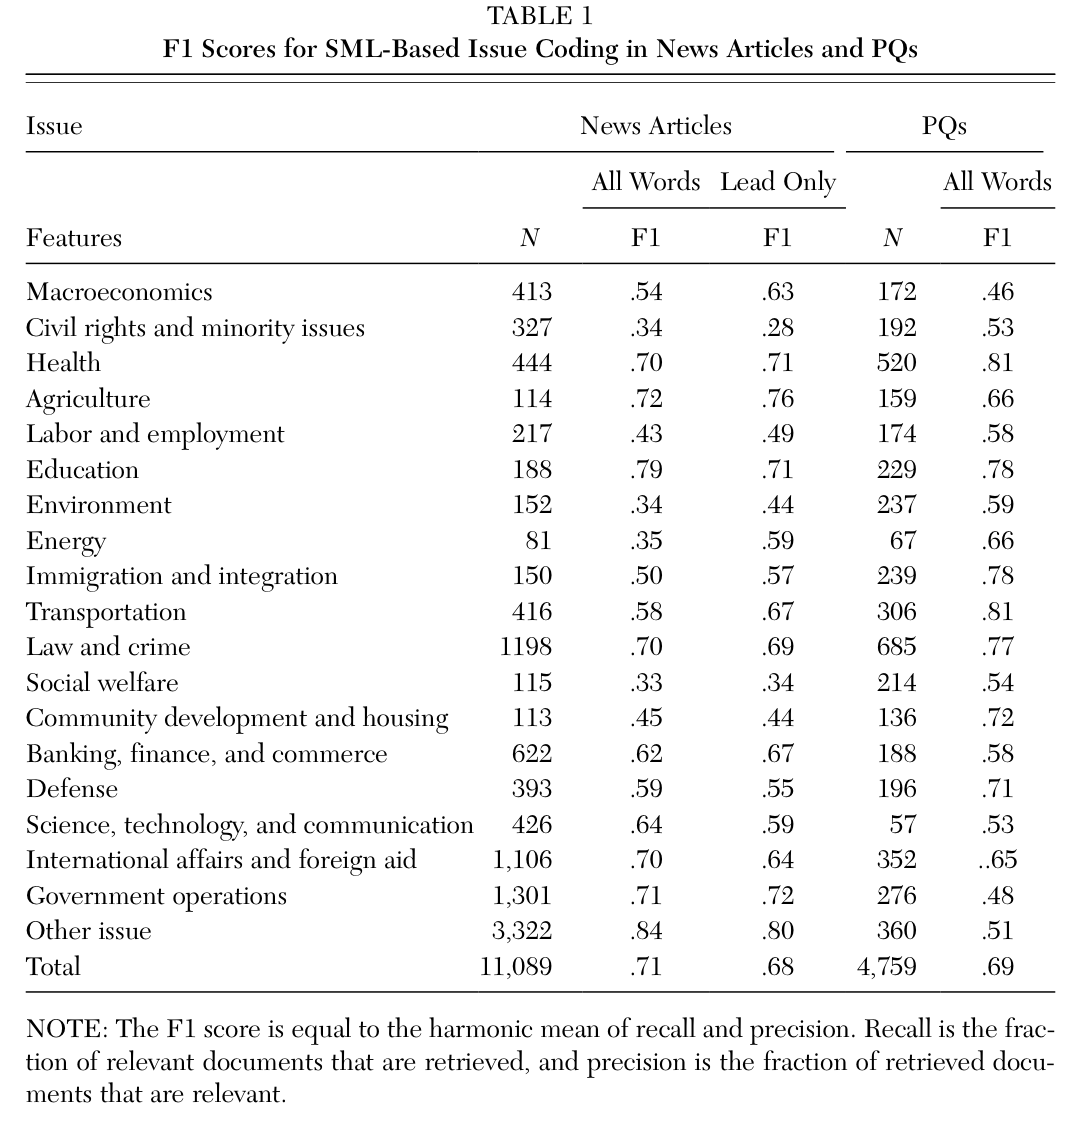
\includegraphics[width=\paperwidth,height=\paperheight,keepaspectratio]{burscher2015-b}}
  \end{frame}
}





\begin{frame}{What does this mean for our research?}
  \begin{block}<2>{It we have 2,000 documents with manually coded frames and topics\ldots}
    \begin{itemize}
    \item we can use them to train a SML classifier
    \item which can code an unlimited number of new documents
    \item with an acceptable accuracy (at least for some of them)
    \end{itemize}
  \end{block}
	\onslide<2>{
	  \tiny{Some easier tasks even need only 500 training documents, see \cite{Hopkins2010}}}.
\end{frame}



\subsection{An implementation}

\begin{frame}[fragile]{An implementation}
Let's say we have a list of tuples with movie reviews and their rating:
\begin{lstlisting}
reviews=[("This is a great movie",1),("Bad movie",-1), ... ...]
\end{lstlisting}
And a second list with an identical structure:
\begin{lstlisting}
test=[("Not that good",-1),("Nice film",1), ... ...]
\end{lstlisting}
Both are drawn from the same population, it is pure chance whether a specific review is on the one list or the other.\\
\tiny{Based on an example from \url{http://blog.dataquest.io/blog/naive-bayes-movies/}}
\end{frame}


\begin{frame}[fragile]{Training a A Naïve Bayes Classifier}
\begin{minted}{python}
from sklearn.naive_bayes import MultinomialNB
from sklearn.feature_extraction.text import CountVectorizer
from sklearn import metrics

# This is just an efficient way of computing word counts
vectorizer = CountVectorizer(stop_words='english')
train_features = vectorizer.fit_transform([r[0] for r in reviews])
test_features = vectorizer.transform([r[0] for r in test])

# Fit a naive bayes model to the training data.
nb = MultinomialNB()
nb.fit(train_features, [r[1] for r in reviews])

# Now we can use the model to predict classifications for our test features.
predictions = nb.predict(test_features)
actual=[r[1] for r in test]

print("Precision: {0}".format(metrics.precision_score(actual, predictions, pos_label=1, labels = [-1,1])))
print("Recall: {0}".format(metrics.recall_score(actual, predictions, pos_label=1, labels = [-1,1])))
\end{minted}
\end{frame}


\begin{frame}{And it works!}
  Using 50,000 IMDB movies that are classified as either negative or positive,
  \begin{itemize}
  \item I created a list with 25,000 training tuples and another one with 25,000 test tuples and
  \item trained a classifier
  \item with precision and recall values $>.80$
  \end{itemize}
  ~\\
  \tiny{Dataset obtained from \url{http://ai.stanford.edu/~amaas/data/sentiment}, Maas, A.L., Daly, R.E., Pham, P.T., Huang, D., Ng, A.Y., \& Potts, C. (2011). Learning word vectors for sentiment analysis. \emph{49th Annual Meeting of the Association for Computational Linguistics (ACL 2011)}
	}
	
\end{frame}

\begin{frame}[fragile]{Playing around with new data}
\begin{minted}{python}
newdata=vectorizer.transform(["What a crappy movie! It sucks!", "This is awsome. I liked this movie a lot, fantastic actors","I would not recomment it to anyone.", "Enjoyed it a lot"])
predictions = nb.predict(newdata)
print(predictions)
\end{minted}
This returns, as you would expect and hope:
\begin{lstlisting} 
[-1  1 -1  1]
\end{lstlisting}


\end{frame}




\begin{frame}{But we can do even better}
  We can use different vectorizers and different classifiers.
\end{frame}


\subsection{Classifiers}


\begin{frame}{Different classifiers}
  Typical options in a nutshell:
  \begin{itemize}
  \item Na\"ive Bayes
  \item Logistic Regression
  \item Support Vector Machine (SVM/SVC)
  \item Random forests
  \end{itemize}
\end{frame}


\subsection{Vectorizers}

\begin{frame}{Different vectorizers}
  \begin{enumerate}[<+->]
  \item CountVectorizer (=simple word counts)
  \item TfidfVectorizer (word counts (``term frequency'') weighted by number of documents in which the word occurs at all (``inverse document frequency''))
  \end{enumerate}
  
	\pause
	$$tfidf_{t,d} = tf_{t,d} \cdot idf_{t}$$
	
	There are different ways to weigh the idf score. A common one is taking the logarithm:
	
	$$idf_{t} = \log \frac{N}{n_t}$$
	
	where $N$ is the total number of documents and $n_t$ is the number of documents containing term $t$
\end{frame}

\begin{frame}{Different vectorizer options}
  \begin{itemize}
  \item Preprocessing (e.g., stopword removal)
  \item Remove words below a specific threshold (``occurring in less than $n=5$ documents'') $\Rightarrow$ spelling mistakes etc.
  \item Remove words above a specific threshold (``occuring in more than 50\% of all documents) $\Rightarrow$ de-facto stopwords
  \item Not only to improve prediction, but also performance (can reduce number of features by a huge amount)
  \end{itemize}
\end{frame}








\begin{frame}{Which one would you (not) use for which purpose?}
	\makebox[\linewidth]{
	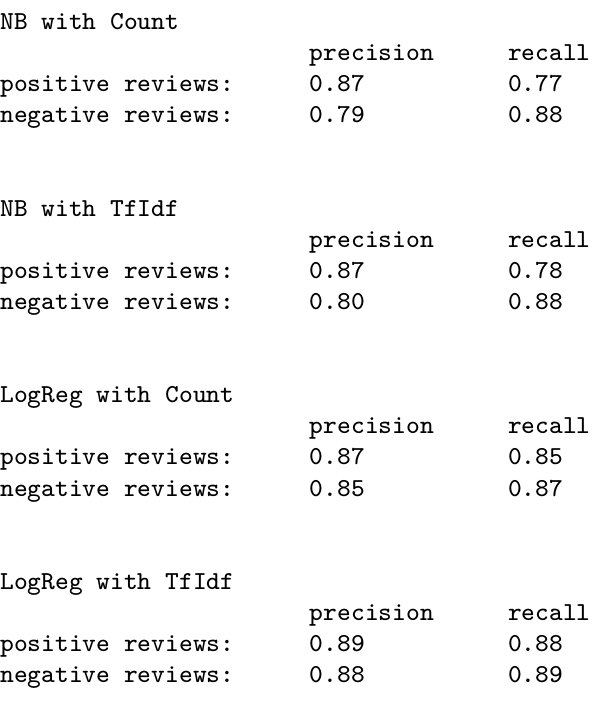
\includegraphics[width=\paperwidth,height=.8\paperheight,keepaspectratio]{imdbsml}}
\end{frame}




\section{Summing up}

\subsection{Revisiting the difference between the dictionary approach and the SML}


\begin{frame}{What \emph{is} our fitted classifier again?}
  Essentially, just a formula 
	
	$$p = \frac{1}{1 + e^{-(\beta_0 + \beta_1 x_1 + \beta_2 x_2 + \ldots + \beta_n x_n)}}$$
	
  where $\beta_0$ is an intercept\footnote{Machine Learning people sometimes call the intercept ``bias'' (yes, I know, that's confusing)}, $\beta_1$ a coefficient for the frequency (or tf$\cdot$ idf score) of some word, $\beta_2$ a coefficient some other word.
	
  If our fitted \emph{vectorizer} contains 5,000 words, we thus have 5,001 coefficients.
	
  \tiny{(for logistic regression in this case, but same argument applies to other classifiers as well)}
	
\end{frame}

\question{But isn't that then essentially very much like a dictionary, except that the words have different weights?}


\begin{frame}{In some sense, yes.}
  \begin{itemize}
  \item But we don't pretend that we can construct the dictionary \emph{a priori}.
  \item It's specifically tailored to our use-case.
  \item The weights are \emph{really} essential here.
  \end{itemize}
  
  \pause
  We \emph{could} print all coefficients-word pairs, but probably it's enough to just look at those with the largest absolute value:
\end{frame}





\begin{frame}{ELI5}
	\makebox[\linewidth]{
	  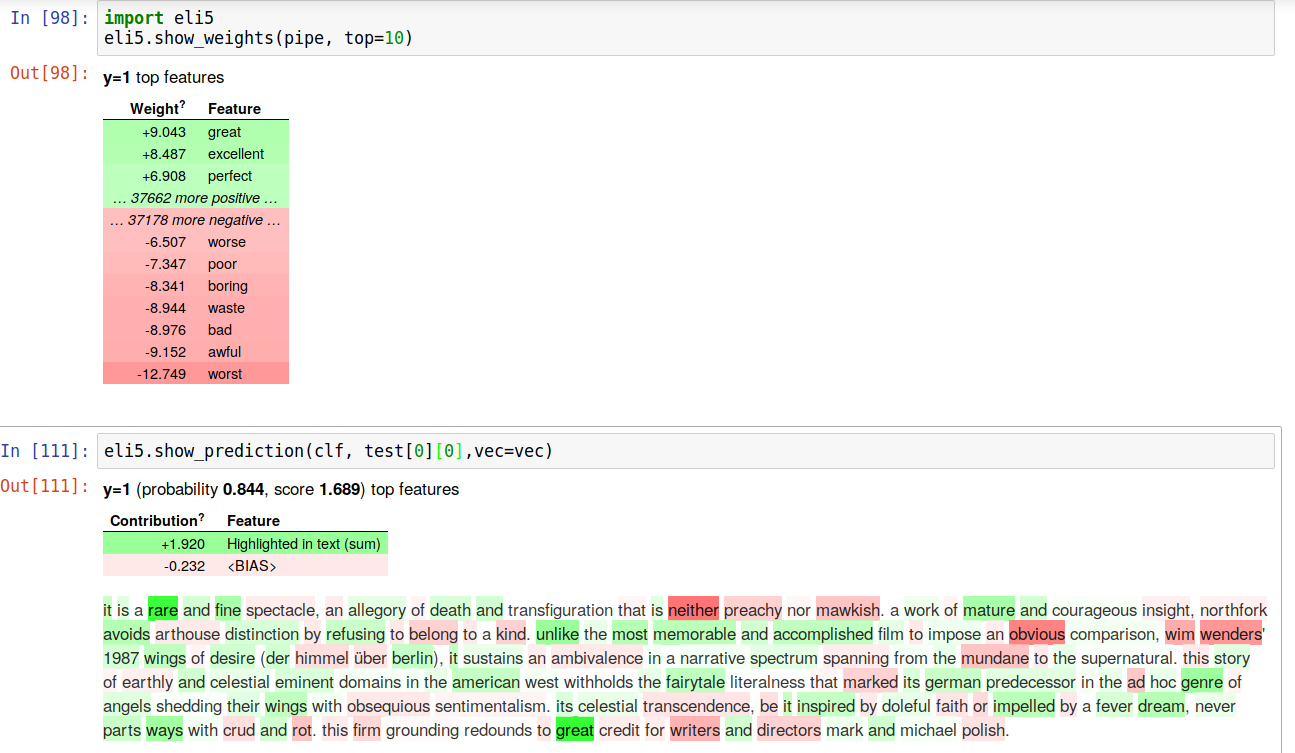
\includegraphics[width=\paperwidth,height=.8\paperheight,keepaspectratio]{eli5}}
\end{frame}

\begin{frame}{ELI5}
  \begin{itemize}
  \item Inspecting \emph{all} coefficients of a ML model usually doesn't make much sense
  \item But that does not mean that we cannot understand how the model makes its predictions
  \item We can look at the most important coefficients
  \item We can look which words in a given text contributed most to its classfication
  \end{itemize}
\end{frame}




\begin{frame}{But have we solved all problems of dictionaries?}
  No.
  
  For instance, the negation and/or intensifier problem.
  
  Possible approaches
  \begin{itemize}
  \item $n$-grams as features
  \item preprocessing (?)
  \item deep learning 
  \item \ldots
  \end{itemize}
  \pause
	
  $\Rightarrow$ \textbf{But ultimately, it's just an empirical question how big the problem is!}
	
	
\end{frame}


\subsection{A note on the input data}

\begin{frame}{The input scikit-learn expects}
  A training dataset consisting of:
  \begin{enumerate}
  \item an array (e.g., a list) of labels (\texttt{y\_train})
  \item a corresponding array (e.g., a list) of feature vectors (\texttt{X\_train})
  \end{enumerate}
	
	A test dataset consisting of:
	\begin{enumerate}
	\item an array (e.g., a list) of labels (\texttt{y\_test})
	\item a corresponding array (e.g., a list) of feature vectors (\texttt{X\_test})
	\end{enumerate}
	
	The feature vectors can be created via a \textit{vectorizer}, but could in principle also just be lists themselves.
	
	We use a lowercase \texttt{y} because it is a onedimensional vector, and an uppercase \texttt{X} because it is a two-dimensional matrix.
\end{frame}


\begin{frame}{The input scikit-learn expects}
  \begin{itemize}
  \item \textbf{It does not matter \emph{how} you create \texttt{y} and \texttt{X}!}
  \item Getting data into the right shape can be as much work (or more) as training the classifier itself
  \end{itemize}
  \pause
  Typical techniques:
  \begin{itemize}
  \item Reading text files from folders into lists of strings (looping over folder contents)
  \item Reading from csv file either directly into lists (\texttt{csv} module) or via pandas
  \item List comprehension to restructure or process data
  \item Potentially, you need to split into train and test dataset yourself (with slicing, or  with scikit-learn itself)
  \end{itemize}
\end{frame}






\begin{frame}{Looking forward: Beyond classic SML}
Note that classic SML is still based on word frequencies with weights (and hence cannot solve all problems we started off with). State-of-the art approaches like deep learning and transformers address this issue -- but that's for another time.
  
\end{frame}










\question{Any questions?}

\begin{frame}{Things to remember}
  \begin{itemize}
  \item unsupervised vs supervised
  \item rough understanding of different techniques and when to use them
  \item evaluation metrics (e.g., precision, recall)
\end{itemize}
\end{frame}

\section{Next steps}

\begin{frame}[standout]
Make sure you understood all of today's concepts.

Re-read the chapters.

On Friday, you will do some machine learning. \large{\url{https://github.com/uvacw/teaching-bdaca/blob/main/12ec-course/week08/exercises/}}

\begin{frame}[plain]
	\printbibliography
\end{frame}


\end{document}
